\subsection*{Equipment}
\addcontentsline{toc}{subsection}{Equipment}
%
"Oh, really, don't you know? These days all it takes for your dreams to come true is money and power."\\   
\indent -- President Shinra
%
\vfill
%
\begin{center} 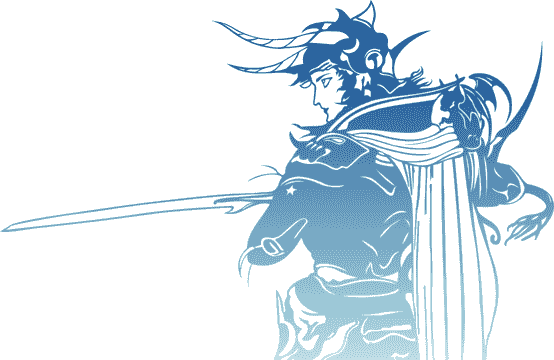
\includegraphics[width=\columnwidth]{./art/images/ff1.png} \end{center}
%
Combat potency can be further improved through \hypertarget{equip}{equipment}. 
While \textbf{weapons} increase the damage dealt, \textbf{armor} protects against incoming damage.
\textbf{Accessories} are miscellaneous pieces that can complement a character's gear.
In addition, all equipment pieces may provide boosts to attributes or other useful effects. 
Every character can wear one weapon, one armor and two accessories. 
Accessories can be worn by everyone, but characters can only equip specific weapon and armor types depending on their job.
Furthermore, characters can use \textbf{Items}, that provide quick benefits in and outside of combat, but are consumed after a single use.
All items and unequipped possessions are stored in your character's \textbf{Inventory}.
%
\vspace{0.5cm}
%
\subsubsection*{Trading}
Equipment and items can be looted from defeated foes and treasure chests or earned as rewards for completing a given task. 
But often the party will need to buy or sell specific things from shops and merchants. 
The currency used for trading is called \textbf{Gil} and typically comes in the form of coins.
You can try buying and selling almost anything, as long as someone is willing to trade.
%
\vfill
%
\example{Trading}{
Terra and her party visit an auction house to bet on rare items.
Today is their lucky day, the item up for bid is a talking \hyperlink{chocobo}{Chocobo}! 
The party is impressed by this talented creature and decides to bid all of their savings, a total of 10000 Gil!
At first it looks like they are outbidding everyone, but in the last second a loving father bids 500000 Gil and acquires the Chocobo as a present for his son.
Maybe the party has better luck (or more money) next time...
}
%
\pagebreak
%
\subsubsection*{Upgrading Equipment}
Weapons and armor can be upgraded to higher Levels to become even more potent.
All equipment pieces start at Level 1 and upgrading them at leasts takes an amount Gil and multiple hours of work.
The GM may enforce additional restrictions on upgrades, such as requiring specific materials or expertise to complete them.
Non-player characters may also upgrade equipment and accordingly higher Level pieces may be found in your world.
An upgraded weapon or armor keeps its special effects, increases in potency and may also change its name or appearance as decided by the upgrader.
There are special rules for some equipment types which are explained in \textbf{notes} in the following.
The tables below shows the costs and effects of upgrading weapons and armor to different Levels.  \\
%
\vfill
%
\begin{tcolorbox}[colback=white,toptitle=0pt,colframe=accent,tabularx={c@{\hspace*{1.2cm}}c@{\hspace*{1.2cm}}l},sharp corners=south,
	title={\hspace*{\fill} \textbf{Weapon Upgrades} \hspace*{\fill}}]	
	\textbf{Level} & \textbf{DMG} & \textbf{Upgrade Cost} \\ \hline
	1 & 1d & 1000 Gil \\ \hline
	2 & 2d & 2000 Gil \\ \hline
	3 & 3d & Cannot be upgraded. \\ \hline
\end{tcolorbox}
%
\vfill
%
\begin{tcolorbox}[colback=white,toptitle=0pt,colframe=accent,tabularx={c@{\hspace*{0.75cm}}c@{\hspace*{0.8cm}}l},sharp corners=south,
	title={\hspace*{\fill} \textbf{Armor Upgrades} \hspace*{\fill}}]	
	\textbf{Level} & \textbf{DEF / RES} & \textbf{Upgrade Cost} \\ \hline
	1 & See notes & 1000 Gil \\ \hline
	2 & +1 / +1 & 2000 Gil \\ \hline
	3 & +1 / +1 & Cannot be upgraded. \\ \hline
\end{tcolorbox}
%
\vfill
%
\subsubsection*{Legendary Equipment}
Apart from normal weapons and armor, there is a special class of equipment that may or may not exist in your world called the \hyperlink{leq}{Legendary Equipment}.
These are extraordinarily powerful weapons and armor with great relevance and accordingly tremendous effort is required to find them.
Legendary Equipment pieces are always unique and cannot be upgraded or upgraded to.
%
\vfill
%
\subsubsection*{Examples}
In the following, some typical equipment pieces and items are shown. 
All weapons have a range of 1u by default.
All Level~1 weapons and armor have a default value of 500 Gil, except for parts that have no unique effects (e.g. \hyperlink{mknife}{Mythril Sword}), which are only worth half as much.
The given lists are not exhaustive and the GM is encouraged to make changes and additions to them.
Usually, the party starts the game with basic equipment (e.g. \hyperlink{mknife}{Mythril Sword}), items (e.g. \hyperlink{item}{Potion}) and some Gil. 
Instead of armor, characters may also wear ordinary clothes which only provide DEF~+1 and cannot be upgraded.
%
\pagebreak
%
\eweapon{Arcos}{weapon.png} {
	\hline Arco \newline de Mithril & -- \\
	\hline Arco \newline Oscuro & Si realizas 3 \hyperlink{action}{Ataques} exitosos sobre un objetivo con esta arma, inflige \hyperlink{status}{Ceguera} por 3 turnos. \\ 
	\hline Arco \newline Élfico & Siempre que realices un \hyperlink{action}{Ataque} sobre un objetivo que tenga algún \hyperlink{status}{Estado Alterado}, añade 1d al daño total. \\  
	\hline Arco \newline Asesino & Si logras hacer \hyperlink{action}{Daño Crítico}, el objetivo pasa instantáneamente a estar \hyperlink{status}{KO}. \\ 
	\hline \multicolumn{2}{p{0.95\columnwidth}}{\textbf{Nota:} Los arcos tienen un alcance de 5u. Si realizas un \hyperlink{action}{Ataque} con un arco, no puedes moverte en ese mismo turno.} }
\vfill
\eweapon{\hypertarget{mknife}{Dagas}}{weapon.png}{
	\hline Cuchillo \newline de Mithril & --\\
   	\hline Daga \newline de Asesino & Si logras hacer \hyperlink{action}{Daño Crítico}, el objetivo pasa instantáneamente a estar \hyperlink{status}{KO}. \\ 
   	\hline Gladius & La DC de todas las tiradas relacionadas con robar se reduce en 1.\\ 
   	\hline Main \newline Gauche & Si hay algún aliado tuyo a 1u del objetivo, añade 1d al daño infligido por \hyperlink{action}{Ataques} con esta arma. \\ 
}
\vfill
\eweapon{Armas de Fuego}{weapon.png} {
	\hline Pistola \newline de Mithril & --  \\ 
	\hline Fomalhaut & El daño infligido por esta arma es del tipo \hyperlink{type}{Mágico}. \\ 
	\hline Metralleta & Cuando realices un \hyperlink{action}{Ataque}, también puedes causar 1d daño a otro enemigo que se encuentre a 1u del objetivo original. \\ 
	\hline Tiny Bee & Después de cada \hyperlink{action}{Ataque}, inmediatamente puedes moverte 1u.\\  
   	\hline \multicolumn{2}{p{0.95\columnwidth}}{\textbf{Nota:} Las pistolas tienen un alcance de 3u. El daño de las armas de fuego no aumenta directamente por la FUE. En su lugar, su daño aumenta 1d por cada 3 puntos de FUE del usuario.} }
\vfill
\eweapon{Puños}{weapon.png}{
	\hline Puños \newline de Mithril & -- \\
	\hline Garra \newline de Gato & La DC de evasión del objetivo aumenta en 1 punto cuando recibe un \hyperlink{action}{Ataque} de esta arma. \\ 
	\hline Puño \newline del Káiser & Si realizas 3 \hyperlink{action}{Ataques} exitosos sobre un objetivo con esta arma, inflige \hyperlink{status}{Inmóvil} por 3 turnos. \\ 
	\hline Colmillos de Tigre & Siempre que el objetivo de tus \hyperlink{action}{Ataques} saque 3 o menos en la tirada de evasión, haces \hyperlink{action}{Daño Crítico}. \\ 
}
\pagebreak
\eweapon{Lanzas}{weapon.png}{
	\hline Lanza \newline de Mithril & --  \\ 
	\hline Gae Bolg & Tienes \hyperlink{check}{Ventaja} en todas las tiradas de iniciativa. \\ 
	\hline Longinus & Si realizas 3 \hyperlink{action}{Ataques} exitosos sobre un objetivo con esta arma, inflige \hyperlink{status}{Veneno} por 3 turnos. \\ 
	\hline Tridente & Esta arma daña al objetivo original y a quien esté directamente detrás de él.\\
	\hline \multicolumn{2}{p{\columnwidth}}{\textbf{Nota:} Las lanzas tienen un alcance de 2u.} }
\vfill
\eweapon{Bastones}{weapon.png}{
	\hline Bastón \newline de Mithril & --  \\ 
	\hline Bastón \newline Elemental & Esta arma debe ser de un elemento específico (p. ej., \hyperlink{type}{Fuego}) y puede tener un nombre acorde (p. ej., "Bastón de Fuego"). Cuando causes daño de ese elemento, añade 1d al total.\\ 
	\hline Bastón \newline Sanador & Cuando cures PV con una habilidad, añade 1d al total. \\ 
	\hline Bastón \newline de Lilith & Puedes evadir los \hyperlink{action}{Ataques} aún cuando estás concentrándote. \\ 
	\hline Bastón \newline de Malboro & Cuando utilices \hyperlink{action}{Magia} que inflija algún \hyperlink{status}{Estado Alterado} negativo, la DC que debe superar el objetivo aumenta 1 punto.\\ 
	\hline Vara \newline Estrellada & Si tienes más de 0 PM, puedes consumir tus PM restantes para lanzar \hyperlink{action}{Magia} con un costo superior al valor que tienes disponible. \\ 
	\hline \multicolumn{2}{p{0.95\columnwidth}}{\textbf{Nota:} Los bastones aumentan un punto de MAG por nivel de arma (por ejemplo, un bastón de Nivel 1 da MAG~+1). A cambio, los bastones no aumentan su daño cuando se mejoran.} }
\vfill
\eweapon{\hypertarget{sword}{Espadas}}{weapon.png}{
	\hline Espada \newline de Mithril & -- \\ 
	\hline Espada Mortal & Cada vez que hagas \hyperlink{action}{Daño Crítico}, haces el cuádruple de daño (en vez del doble). \\ 
	\hline Sable-pistola & Siempre que utilices una habilidad, puedes hacer un \hyperlink{action}{Ataque} adicional a distancia con un alcance de 3u. Para este Ataque, no sumas tu FUE al daño.\\ %L6
	\hline Joyeuse & Siempre que inflijas un \hyperlink{status}{Estado Alterado}, aumenta 1 turno a su duración. \\
	\hline Organyx & Cuando hagas un \hyperlink{action}{Ataque} sobre un enemigo, recuperas 1d de PM. \\
	\hline Viva \newline la Reina & Cuando tú o un aliado a 1u de distancia sea dañado por \hyperlink{action}{Magia}, puedes reducir el daño a la mitad si pasas una DC de 9. \\ 
}
\pagebreak
\earmor{Armadura Pesada}{armor.png}
{
	\hline Armadura \newline Mithril & --  \\ 
	\hline Malla \newline de Cristal & Resiste: \hyperlink{type}{Hielo} \\
	\hline Malla\newline de Demonio & Resiste: \hyperlink{type}{Oscuro} \\ 
	\hline Armadura\newline de Diamante & Resiste: \hyperlink{type}{Eléctrico} \\ 
	\hline Malla \newline de Dragón & Resiste: \hyperlink{type}{Eléctrico} \\ 
	\hline Armadura\newline de Caballero & FUE +1 \\ 
	\hline Malla \newline de Espejo & Inmunidad: \hyperlink{status}{Silencio} \\
	\hline \multicolumn{2}{p{0.95\columnwidth}}{\textbf{Nota:} Toda armadura pesada proporciona DEF +2 en el nivel 1 de armadura.}
}
\vfill
\earmor{Armadura Ligera}{armor.png}
{
	\hline Chaleco \newline de Mithril & -- \\ 
	\hline Equipo de Gaia & Resiste: \hyperlink{type}{Tierra} \\
	\hline Traje Kenpogi & Inmunidad: \hyperlink{status}{Ceguera} \\ 
	\hline Minerva & Resiste: \hyperlink{type}{Hielo} \\
	\hline Chaleco de \newline Espejismo & Inmunidad: \hyperlink{status}{Sueño} \\ 
	\hline Equipo de Ninja & Inmunidad: \hyperlink{status}{Inmóvil} \\ 			 
	\hline Chaleco \newline de Poder & FUE +1 \\ 
	\hline Chaqueta Roja & Resiste: \hyperlink{type}{Fuego} \\ 
	\hline Chaleco de \newline Supervivencia & +5 a los PV máximos \\ 
	\hline \multicolumn{2}{p{0.95\columnwidth}}{\textbf{Nota:} Toda armadura ligera proporciona DEF +1 y RES +1 en el nivel 1 de armadura.} }
\vfill
\earmor{Túnicas}{armor.png}
{
	\hline Túnica \newline de Seda &  --  \\
	\hline Túnica \newline Negra & Inmunidad: \hyperlink{status}{Veneno} \\
	\hline Túnica de \newline Algodón & Resiste: \hyperlink{type}{Viento} \\ 
	\hline Túnica \newline Luminosa & Resiste: \hyperlink{type}{Sagrado} \\ 
	\hline Túnica \newline de Mago & MAG +1 \\ 
	\hline Túnica \newline de Erudito & +5 a los PM máximos \\
	\hline Túnica \newline Blanca & Inmunidad: \hyperlink{status}{Sueño} \\  
	\hline \multicolumn{2}{p{0.95\columnwidth}}{\textbf{Nota:} Todas las túnicas proporcionan RES +2 en el nivel 1 de armadura.} }
\pagebreak
\lweapon{\hypertarget{leq}{Armas Legendarias}}{weapon.png} {
	\hline Arma \newline Omega & Cualquiera & +10 a los PV máximos. \newline Esta arma puede ser de cualquier tipo (p. ej. Espada). \\ 
	\hline Arma \newline Artema & Cualquiera & +10 a los PM máximos. \newline Esta arma puede ser de cualquier tipo (p. ej. Espada). \\  
	\hline Artemisa & Arco & Los \hyperlink{action}{Ataques} que provengan de este arco no pueden ser esquivados. \\ 
	\hline Matamagos & Daga & Reduce los PM del objetivo en la misma cantidad que los PV de daño infligidos. \\ 	
	\hline Pena \newline de Muerte & Arma de \newline Fuego & Cuando inflijas el estado \hyperlink{status}{KO} a un enemigo, puedes hacer inmediatamente otro \hyperlink{action}{Ataque}.\\
	\hline Mano \newline de Dios & Puño & El daño infligido por esta arma es del tipo \hyperlink{type}{Mágico} y \hyperlink{type}{Sagrado}. \\  
	\hline Gungnir & Lanza & Cuando caes sobre un enemigo luego de un Salto, infliges 1d de daño \hyperlink{type}{Eléctrico}. \\
	\hline Nirvana & Bastón & Cuando lanzas \hyperlink{action}{Magia} que inflige daño o recupera PV, obtienes 1d adicional. \\
	\hline Maza \newline de Zeus & Bastón & Cuando lanzas \hyperlink{action}{Magia} con éxito, recuperas 1d de PM. \\    
	\hline Excalibur & Espada & Al atacar, añade 1d de daño \hyperlink{type}{Sagrado}. \\ 	
	\hline Masamune & Espada & Los daños provocados por esta arma ignoran \hyperlink{type}{Resistencia}. \\ 	
	\hline Ragnarok & Espada & Cuando tus PV están por debajo del 10 \% de su valor máximo, cada \hyperlink{action}{Ataque} exitoso contra un enemigo hace \hyperlink{action}{Daño Crítico} \\ 
	\hline \multicolumn{3}{p{0.95\columnwidth}}{\textbf{Nota:} Todas las armas legendarias infligen 4d de daño y están sujetas a las reglas específicas de su tipo.} }
\vfill
\lweapon{Armadura legendaria}{armor.png}{ 
	\hline Armadura Genji & Armadura Pesada & FUE +2 \\ 
	\hline Maximillian & Armadura Pesada & +10 a los PV máximos. \\ 
	\hline Atuendo \newline Negro & Armadura ligera & Tienes \hyperlink{check}{Ventaja} en todas las tiradas de iniciativa. \\ 
	\hline Traje \newline de Héroe & Armadura ligera & Todos los beneficios recibidos de \hyperlink{status}{aumATR} se duplican.\\ 	
	\hline Túnica de los Señores & Túnica & Resiste: \hyperlink{type}{Daño elemental} \\ 
	\hline Túnica \newline de Sabio & Túnica & +10 a los PM máximos \\ 
	\hline \multicolumn{3}{p{0.95\columnwidth}}{\textbf{Nota:} Todas las armaduras legendarias otorgan +4 a DEF y RES.} }

\accessory{Accessories}{acc.png}
{
	\hline Mythril Shield & 500 Gil & DEF +1  \\ 
    \hline Power Armlet & 500 Gil & STR +1 \\ 
    \hline Rune \newline Bracers & 500 Gil & RES +1 \\
   	\hline Battle Boots & 750 Gil & Immunity: \hyperlink{status}{Immobile}  \\
 	\hline Silver Glasses & 750 Gil & Immunity: \hyperlink{status}{Blind}  \\   
	\hline Star \newline Pendant & 750 Gil & Immunity: \hyperlink{status}{Poison}  \\
	\hline White Cape & 750 Gil & Immunity: \hyperlink{status}{Silence}  \\ 	
	\hline Thief Gloves & 1000 Gil & You have \hyperlink{check}{Advantage} on all checks related to \hyperlink{thief}{stealing}. \\ 
    \hline Protect Ring & 1250 Gil & Whenever you suffer an \hyperlink{action}{Attack}, you gain \hyperlink{status}{EnDEF} for 1 round.\\
    \hline Circlet & 1500 Gil & RES +1, MAG +1\\
    \hline Grand \newline Helmet & 1500 Gil & STR +1, DEF +1\\  
    \hline Safety Bit & 1500 Gil & Immunity: \hyperlink{status}{KO}  \\ 
    \hline Champion Belt & 2000 Gil & STR +1, \newline Immunity: \hyperlink{status}{DeATR} \\ 
    \hline Germinas Boots & 2500 Gil & You can jump twice as high as usual.  \\  
   	\hline Black Belt & 3000 Gil & Maximum HP +10  \\ 
   	\hline Moogle Charm & 4000 Gil & Glows when there is a monster within 50u of you.  \\  
    \hline Hero's Shield & 5000 Gil & DEF +1, RES +1, \newline Immunity: \hyperlink{status}{Sleep}\\
    \hline Feather Boots & 6000 Gil & You can levitate up to 1u above the ground. \\
    \hline Hermes Sandals & 7000 Gil & AGI~+1 \\
    \hline Genji \newline Helmet & 9000 Gil & Resilience: \hyperlink{type}{magical}\\  
    \hline Genji Shield & 9000 Gil & Resilience: \hyperlink{type}{physical}\\ 
   	\hline Genji Gloves & 9999 Gil & Whenever you make an \hyperlink{type}{Attack}, you can make a second one immediately after.  \\ 
   	\hline Ribbon & 9999 Gil & Immunity: \hyperlink{status}{All Status Effects}  \\
   	\hline Gold \newline Hairpin & 9999 Gil & Whenever you use \hyperlink{action}{Magic}, the MP cost is halved.  \\  
   	\hline Dragon Seal & ??? Gil & Proof of slaying a dragon god. \\
   	\hline Omega Badge & ??? Gil & Proof of defeating an ancient weapon. \\ 
	\hline \multicolumn{3}{p{0.95\columnwidth}}{\textbf{Note:} For some accessories it does not make sense to wear two of the same type (e.g. shields).}
}
\consumables{Items}{item2.png}
{
	\hline Gysahl Greens & 25 Gil & Vegetable well-known as a \hyperlink{chocobo}{Chocobo's} favorite food. \\
	\hline Antidote & 50 Gil & Removes \hyperlink{status}{Poison}.\\ 
	\hline Eyedrops & 50 Gil & Removes \hyperlink{status}{Blind}.  \\ 
	\hline Echo Grass & 50 Gil & Removes \hyperlink{status}{Silence}.  \\ 
	\hline Gold \newline Needle & 50 Gil & Remove \hyperlink{status}{Immobile}. \\ 
	\hline Arctic Wind & 100 Gil & The target suffers 2d \hyperlink{type}{ice} damage. \\
	\hline Bomb Fragment & 100 Gil & The target suffers 2d \hyperlink{type}{fire} damage.  \\
	\hline Lightning Gem & 100 Gil & The target suffers 2d \hyperlink{type}{lightning} damage. \\ 
	\hline Potion & 100 Gil & The target regains 2d HP.  \\ 
	\hline Holy\hspace{0.05cm}Water & 150 Gil & Removes \hyperlink{status}{Zombie}.  \\
	\hline Light \newline Curtain & 200 Gil & The target gains \hyperlink{status}{EnDEF} for 3 rounds. \\
	\hline Lunar \newline Curtain & 200 Gil & The target gains \hyperlink{status}{EnRES} for 3 rounds.  \\
	\hline Malboro Vine & 250 Gil & The target makes a DC 8 check and suffers \hyperlink{status}{Poison} for 3 rounds upon failure. \\
	\hline Remedy & 250 Gil & Removes all status effects, except \hyperlink{status}{KO}.  \\ 
	\hline Sleeping Powder & 250 Gil & The target makes a DC 8 check and suffers \hyperlink{status}{Sleep} for 3 rounds upon failure. \\
	\hline Ether & 300 Gil & The target regains 2d MP.\\ 	
	\hline Hero Drink & 300 Gil & The target gains \hyperlink{status}{EnSTR} and \hyperlink{status}{EnMAG} for 3 rounds. \\
	\hline Warp Stone & 300 Gil & You teleport to a place you can see within 10u. \\
	\hline Hi-Potion & 400 Gil & The target regains 6d HP.  \\ 
	\hline Phoenix Down & 500 Gil & Removes \hyperlink{status}{KO} and the target regains 1 HP.\\ 
	\hline Dark \newline Matter & 500 Gil & The target suffers 8d \hyperlink{type}{dark} damage \\
	\hline Turbo Ether & 750 Gil & The target regains 6d MP. \\
	\hline Mega-Potion & 800 Gil & Everyone within 1u regains 6d HP.  \\  
	\hline Elixir & 1000 Gil & The targets fully regains HP and MP. \\ 
	\hline Tent & 1000 Gil & Allows the party to sleep outside comfortably. \\
	\hline Gold \newline Hourglass & 1500 Gil & Time freezes for everyone except yourself within 5u for 20 seconds (2 rounds).  \\
	\hline Mega-Elixir & 2000 Gil & Everyone within 1u fully regains their HP and MP. \\
	\hline Mega-Phoenix & 3000 Gil & Removes \hyperlink{status}{KO} from everyone within 1u and fully recovers their HP and MP. \\
}
\pagebreak
\twocolumn

